\documentclass[letterpaper]{article} % DO NOT CHANGE THIS
\usepackage[submission]{aaai2027}  % DO NOT CHANGE THIS
\usepackage[hyphens]{url}  % DO NOT CHANGE THIS
\usepackage{graphicx} % DO NOT CHANGE THIS
\urlstyle{rm} % DO NOT CHANGE THIS
\def\UrlFont{\rm}  % DO NOT CHANGE THIS
\usepackage{natbib}  % DO NOT CHANGE THIS AND DO NOT ADD ANY OPTIONS TO IT
\usepackage{caption} % DO NOT CHANGE THIS AND DO NOT ADD ANY OPTIONS TO IT
\frenchspacing  % DO NOT CHANGE THIS
\usepackage{amsmath}
\usepackage{amssymb}
\usepackage{array}
\usepackage{booktabs}
\usepackage{multirow}
\usepackage{tabularx}

\pdfinfo{
/TemplateVersion (2027.1)
}

\setcounter{secnumdepth}{0}
\raggedbottom

\title{Adaptive Proximal Control for Federated Personalization}

\author{
    Anonymous Submission
}
\affiliations{
}

\begin{document}

\maketitle

\begin{abstract}
Regularization-based federated personalization methods such as Ditto rely on a fixed proximal coefficient to control how strongly client models remain coupled to a shared global model. This coefficient is not deployment-stable: in our experiments, the best value changes across data regimes and participation rates, so a value tuned before deployment can become stale after conditions shift---a failure we call \emph{coefficient staleness}. We introduce AdaDitto, which treats proximal strength as a bounded online control variable and updates each client's coefficient from a clipped loss-gap signal available during training, while preserving Ditto's objective form and model-update communication pattern. Across CIFAR-100 image classification and Shakespeare next-character prediction, fixed coefficients exhibit distinct regimes; most importantly, on the pathological CIFAR-100 split, the full-participation optimum $\lambda=0$ becomes stale under 20\% participation, where AdaDitto increases coupling online and improves over the frozen baseline by 1.8 points, with larger gains in the client tail. AdaDitto remains below a per-condition oracle that re-tunes the coefficient for each setting, so its contribution is not oracle replacement but reduced dependence on repeated coefficient sweeps under deployment shift.
\end{abstract}

\begin{links}
    \link{Code}{https://anonymous.4open.science/r/PFLlib-5B8C}
\end{links}

\section{Introduction}

Federated learning is commonly built around repeated local client
optimization and server aggregation, as in
FedAvg~\cite{mcmahan2017communication}. Under heterogeneous client
data, however, local updates can drift away from globally useful
directions and aggregation can reflect mismatched local
objectives~\cite{karimireddy2020scaffold,wang2020fednova}.
Regularization-based federated learning methods control the relation
between local adaptation and global sharing through a proximal term.
FedProx~\cite{li2020federated} penalizes local drift from the current
global model, while Ditto~\cite{li2021ditto} trains personalized
client models around a shared global model. In both cases, a single
scalar coefficient ($\mu$ in FedProx, $\lambda$ in Ditto) governs the
strength of this constraint and mediates the trade-off between global
consistency and local adaptation.

That scalar is usually selected by an offline sweep. We ask whether a
coefficient selected under one deployment condition remains reliable
when the participation rate, heterogeneity regime, or active client
population changes. Our fixed-Ditto sweeps show that it need not. We
call this failure mode \emph{coefficient staleness}: a coefficient that
performs well in its tuning condition becomes suboptimal after
deployment conditions shift.

This failure appears directly in our fixed-Ditto sweeps. On the
CIFAR-100 pathological split, full participation selects pure-local
Ditto, with $\lambda=0$, while reducing participation to 20\% moves the
best fixed coefficient to nonzero coupling. Freezing the
full-participation value therefore produces coefficient staleness under
the new participation regime.

We study proximal strength as a bounded online control variable rather
than a fixed hyperparameter. From a control perspective, the proximal
coefficient acts like a gain: a fixed value trades off stability and
responsiveness across operating regimes. But client drift changes
during training and across deployment conditions, while the proximal
constraint is usually kept static. AdaDitto updates each client's
coefficient from a clipped loss-gap signal comparing the received
global model's local probe loss to a server reference. The controller
uses only scalar quantities available during training, preserves the
underlying proximal objective form, and adds one scalar loss report per
participating client plus one scalar reference in the server
broadcast.

The comparison we target is deployment shift, not hindsight tuning. A
fixed Ditto coefficient may be selected under one participation regime
and then deployed under another without the luxury of a fresh sweep.
AdaDitto is designed for this tune-once setting. In our experiments,
it recovers part of the loss caused by a stale full-participation
coefficient under CIFAR-100 pathological participation shift, while
remaining below fixed Ditto when the latter is re-tuned separately for
each condition. The controller should therefore be read as a
retuning-reduction mechanism rather than an oracle replacement.

\paragraph{Contributions.}
We make three contributions. First, we frame proximal coefficient
selection as a deployment-stability problem and distinguish
per-condition oracle tuning from tune-once deployment. Second, we
introduce a bounded loss-gap controller for proximal personalization,
instantiated in AdaDitto, that adapts the proximal coefficient without
changing the underlying objective form or model-update communication
pattern. Third, we show that fixed Ditto coefficients are regime- and
participation-dependent across CIFAR-100 and Shakespeare, and that
AdaDitto reduces coefficient staleness under CIFAR-100 pathological
participation shift while exposing its limits against oracle retuning.

\section{Related Work}

Under heterogeneous client data, local federated updates can drift or
optimize objectives that are mismatched with the intended global
objective. FedAvg~\cite{mcmahan2017communication} provides the
canonical local-optimization and server-aggregation baseline.
FedProx~\cite{li2020federated} adds a proximal penalty to limit local
movement from the current global model,
SCAFFOLD~\cite{karimireddy2020scaffold} uses control variates to
correct client drift, FedNova~\cite{wang2020fednova} normalizes
aggregation to address objective inconsistency, and
FedDyn~\cite{acar2021feddyn} introduces dynamic regularization to
align local and global solutions. AdaDitto is closest to the
regularization line, but adapts the existing Ditto proximal coefficient
rather than changing aggregation, adding control variates, or
introducing a new global correction term.

Personalized federated learning relaxes the goal of learning one model
for all clients. Early federated multi-task methods such as
MOCHA~\cite{smith2017federated} treat clients as related but distinct
tasks. Regularization-based methods such as
pFedMe~\cite{dinh2020personalized} and Ditto~\cite{li2021ditto}
couple personalized models to shared global structure through a penalty
term. Other approaches personalize by learning mixtures of local and
global models~\cite{deng2020adaptive}, adapting a global
initialization~\cite{fallah2020personalized}, separating shared and
client-specific layers~\cite{arivazhagan2019federated,collins2021exploiting},
or keeping batch-normalization statistics local under feature
shift~\cite{li2021fedbn}. AdaDitto belongs to the
regularization-based family: it preserves Ditto's personalized
objective and changes only the scalar coupling strength online.

The practical weakness of fixed-$\lambda$ personalization is that
coefficient choice is deployment-dependent. Selecting $\lambda$ by an
offline sweep is costly in federated learning because each candidate
may require a distributed run, and noisy partial participation can make
validation-based selection unreliable~\cite{kuo2023noisy,wang2023fedhpo}.
A fixed coefficient is therefore not only a tuning choice; it is an
assumption that the participation regime, heterogeneity structure, and
active client population remain close to the condition under which the
sweep was performed.

Adaptive federated methods have adjusted server optimizers,
aggregation, client learning rates, local training schedules, client
participation, and personalization weights in response to observed
training signals~\cite{reddi2021adaptive,kim2024adaptive,sun2023fedlalr,wu2023faster,shenaj2025adaptive,deng2020adaptive}.
These methods adapt important parts of the federated pipeline, but they
do not directly treat the proximal coefficient as the online control
variable. AdaDitto instead adapts the scalar coupling strength between
personalized and global models while preserving Ditto's objective form
and model-update communication pattern.

\section{Methodology}
\label{sec:methodology}

\paragraph{Interpreting proximal sweeps.}
The Ditto coefficient~$\lambda$ determines which information source a
personalized model trusts during local adaptation. When $\lambda$ is
small, the client model can specialize almost independently of the
global model. When $\lambda$ is large, the client model is pulled
toward the shared model and uses global structure as an anchor. Thus
a $\lambda$ sweep is a diagnostic of the coupling regime:
$\lambda=0$ means the best strategy is effectively pure local
personalization, while a nonzero optimum means that local adaptation
benefits from shared anchoring. A deployment shift is harmful when it
changes this coupling regime after $\lambda$ has already been
selected.

We consider clients $\mathcal{C}=\{1,\dots,N\}$, where client $i$ has empirical objective $F_i$. At round $t$, the server broadcasts global parameters $w^{(t)}$ to a sampled subset $\mathcal{S}_t$. Participating clients update the global model for aggregation while maintaining personalized models locally.

\subsection{Ditto Baseline}

Ditto trains each personalized model $v_i$ around the current global model using
\begin{equation}
\label{eq:ditto_obj}
\min_{v_i}\; F_i(v_i) + \frac{\lambda}{2}\|v_i-w^{(t)}\|^2.
\end{equation}

The coefficient $\lambda$ controls the coupling between the personalized and global models: small $\lambda$ permits stronger local adaptation, while large $\lambda$ keeps $v_i$ closer to $w^{(t)}$. In standard Ditto, $\lambda$ is fixed throughout training. AdaDitto replaces it with a client-specific online coefficient $\lambda_i^{(t)}$.

\subsection{Loss-Gap Controller}

At round $t$, the server broadcasts $w^{(t)}$ and the previous scalar loss reference $L_g^{(t-1)}$. Before local training, each participating client evaluates the received global model on a small local probe minibatch $\mathcal{B}_i^{(t)}$:
\begin{equation}
\label{eq:probe_loss}
\hat{L}_i^{(t)}
=
\frac{1}{|\mathcal{B}_i^{(t)}|}
\sum_{(x,y)\in\mathcal{B}_i^{(t)}}
\ell(w^{(t)};x,y).
\end{equation}

The client compares this probe loss to the server reference using a nonnegative clipped log gap:
\begin{equation}
\label{eq:gap}
g_i^{(t)} =
\mathrm{clip}\left(
\log\frac{\hat{L}_i^{(t)}+\epsilon}{L_g^{(t-1)}+\epsilon},\; 0,\; \tau
\right).
\end{equation}

The loss gap is used as a stress signal, not as a claim that the
current global model is already good for that client. A large positive
gap means that the received global model performs worse on client $i$
than on the server reference population. In the participation-shift
regimes we target, this gap empirically coincides with conditions where
stronger anchoring is beneficial. AdaDitto responds by increasing the stabilizing proximal anchor,
limiting unconstrained local drift while still allowing personalization
through the local objective. The response is deliberately bounded: the
controller can increase coupling when the gap rises, but clipping
prevents a single noisy probe from dominating training.

The gap is mapped to a target coefficient and smoothed:
\begin{align}
\lambda_i^{\ast(t)} &= \lambda_{\mathrm{base}} + \alpha g_i^{(t)}, \\
\tilde{\lambda}_i^{(t)} &= (1-\gamma)\lambda_i^{(t-1)} + \gamma\lambda_i^{\ast(t)}, \\
\lambda_i^{(t)} &= \mathrm{clip}(\tilde{\lambda}_i^{(t)},\lambda_{\min},\lambda_{\max}).
\end{align}

The client then updates its personalized model using Eq.~\ref{eq:ditto_obj} with $\lambda$ replaced by $\lambda_i^{(t)}$, and returns its usual global-model update together with the scalar probe loss. The server updates the reference for future rounds using a median exponential moving average:
\begin{equation}
\label{eq:global_loss}
L_g^{(t)} =
\beta L_g^{(t-1)}
+
(1-\beta)\cdot
\mathrm{median}\big(\{\hat L_i^{(t)}\}_{i\in\mathcal{S}_t}\big).
\end{equation}

AdaDitto changes only the proximal coefficient used for personalized training. The personalized model remains local, the global-model update and aggregation procedure are unchanged, and the extra communication is one scalar probe loss per participating client plus one scalar reference in the server broadcast. Since the gap and final coefficient are clipped, $\lambda_i^{(t)}\in[\lambda_{\min},\lambda_{\max}]$ for all clients and rounds.

\paragraph{Controller defaults.}
Unless otherwise stated, all main comparisons use the controller
configuration in Table~\ref{tab:controller-defaults}, without
condition-specific search. We additionally use $\epsilon=10^{-8}$,
a two-round warmup, and at least one probe example.

\begin{table}[t]
\centering
\scriptsize
\setlength{\tabcolsep}{4pt}
\renewcommand{\arraystretch}{1.08}
\begin{tabularx}{\columnwidth}{@{}lX@{}}
\toprule
Controller item & Value or rule \\
\midrule
Base / range & $0.08$ with clipping to $[0.05,3.0]$ \\
Gain / gap cap & $\alpha=0.8$, $\tau=0.7$ \\
Smoothing & coefficient EMA $\gamma=0.3$, reference EMA $\beta=0.9$ \\
Probe & 10\% local examples, cap 256, pre-training inference \\
Communication & one scalar loss up, one scalar reference down \\
\bottomrule
\end{tabularx}
\caption{Default AdaDitto controller configuration used in all main comparisons.}
\label{tab:controller-defaults}
\end{table}

\section{Experimental Design}
\label{sec:experimental}

We design the experiments around a deployment question: when
heterogeneity or participation changes, does a fixed Ditto coefficient
remain reliable, and can AdaDitto reduce the need to re-tune it? Each
experiment therefore varies one of two stressors: the statistical
regime induced by the client partition, and the fraction of clients
participating in each round.

The evaluation uses CIFAR-100~\cite{krizhevsky2009learning} for image
classification and Shakespeare from LEAF~\cite{caldas2018leaf} for
next-character prediction. CIFAR-100 gives controlled regimes: a
Dirichlet split with overlapping but unbalanced labels, which we call
\emph{practical}, and a label-shard split with stronger client
specialization, which we call \emph{pathological}. Shakespeare provides
a naturally federated text regime in which clients correspond to
speaking roles. The reported metric is personalized-model accuracy.
We report personalized-model accuracy because Ditto and AdaDitto optimize client-specific personalized models; tail metrics such as client-unweighted 10th-percentile and worst-client accuracy are used to check whether average gains hide client-level failures.

Table~\ref{tab:evaluation-regimes} summarizes the evaluation
regimes and the role each plays in testing coefficient stability.
In the pathological CIFAR-100 split, 20 clients each receive
10 labels, so every class appears on two clients.

\begin{table}[ht]
\centering
\scriptsize
\setlength{\tabcolsep}{3pt}
\renewcommand{\arraystretch}{1.08}
\begin{tabularx}{\columnwidth}{@{}>{\raggedright\arraybackslash}p{0.26\columnwidth}>{\raggedright\arraybackslash}p{0.22\columnwidth}>{\raggedright\arraybackslash}p{0.18\columnwidth}>{\raggedright\arraybackslash}X@{}}
\toprule
Setting & Partition & Participation & Role in evaluation \\
\midrule
CIFAR practical &
Dirichlet, $\alpha=0.1$ &
Full, 50\%, 20\% &
Overlapping-label regime for coefficient stability. \\
CIFAR pathological &
Label shard &
Full, 50\%, 20\% &
High-heterogeneity regime for participation-shift stress tests. \\
Shakespeare &
Speaker split &
10\%; 50\% ref. &
Text regime checking whether nonzero coupling is beneficial. \\
\bottomrule
\end{tabularx}
\caption{Evaluation regimes and their roles in the deployment-stability study.}
\label{tab:evaluation-regimes}
\end{table}

We compare fixed Ditto and AdaDitto under identical models, client
sampling, local training budgets, and evaluation code. For fixed
Ditto, we distinguish two standards. A \emph{per-condition tuned}
baseline re-sweeps $\lambda$ for each dataset and participation level;
this is an oracle-style comparison and is not meant to represent
deployment without retuning. A \emph{tune-once} baseline selects
$\lambda$ under full participation and then freezes it under lower
participation. This second standard tests coefficient staleness under
deployment shift.

The sweep grids and replication roles are listed in
Table~\ref{tab:sweep-protocol}.

\begin{table}[t]
\centering
\scriptsize
\setlength{\tabcolsep}{3pt}
\renewcommand{\arraystretch}{1.08}
\begin{tabularx}{\columnwidth}{@{}>{\raggedright\arraybackslash}p{0.29\columnwidth}>{\raggedright\arraybackslash}Xc@{}}
\toprule
Experiment role & Grid or comparison rule & Replication \\
\midrule
CIFAR full sweeps &
\begin{tabular}[t]{@{}l@{}}
$\{0,.001,.005,.01,.03,.05,.08,$\\
$.1,.2,.5,1,2,3\}$
\end{tabular} &
1 seed \\
CIFAR partial sweeps &
$\lambda\in\{0,10^{-3},10^{-2},0.1,0.5,1\}$ &
1 seed \\
Shakespeare sweeps &
$\lambda\in\{0,0.1,0.5,1\}$ at 10\% and 50\% participation &
1 seed \\
Tune-once shift &
tune under full participation, then freeze after shift &
3 seeds \\
CIFAR core comparisons &
select $\lambda$ by per-condition sweep, then evaluate selected Ditto and AdaDitto &
5 seeds \\
Controller stress &
vary controller settings around default &
3 seeds/config \\
\bottomrule
\end{tabularx}
\caption{Sweep grids and replication rules. Single-seed sweeps identify coefficient regimes; multi-seed comparisons estimate robustness for the main claims.}
\label{tab:sweep-protocol}
\end{table}

\section{Results}

The results support a conditional deployment-stability claim.
Fixed Ditto coefficients are not stable across regimes and
participation rates, and a coefficient tuned under one condition
can become stale when participation changes. AdaDitto reduces
coefficient staleness under CIFAR-100 pathological participation
shift, but it does not replace per-condition oracle retuning. We
therefore organize the results by evaluation standard: fixed
coefficient sweeps, tune-once deployment, controller behavior,
controller sensitivity, loss-gap mechanism, and oracle/null comparisons.
We use fixed-$\lambda$ sweeps to diagnose the preferred coupling
regime, per-condition tuned Ditto as a hindsight oracle, tune-once
Ditto to measure coefficient staleness, and AdaDitto to test whether
online control reduces that staleness without a new sweep.

\begin{figure*}[t]
  \centering
  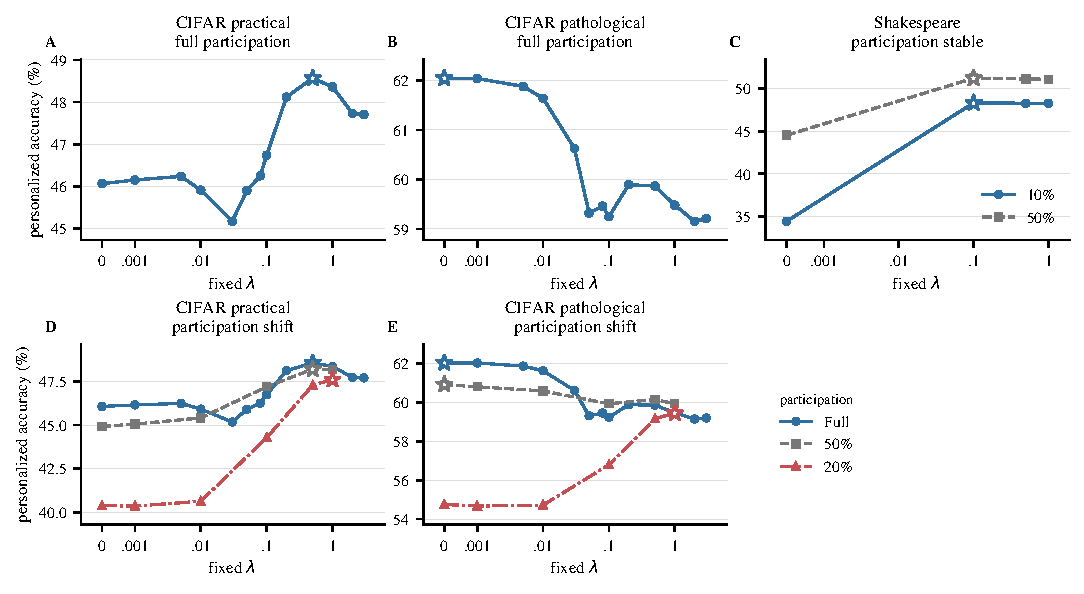
\includegraphics[width=0.90\textwidth]{Figures/current/lambda_stress_grid.pdf}
  \caption{Fixed Ditto coefficients are not deployment-stable. The best $\lambda$ depends on both heterogeneity regime and participation rate: CIFAR-100 practical favors nonzero coupling, CIFAR-100 pathological under full participation favors $\lambda=0$, and Shakespeare requires nonzero coupling throughout. The key deployment failure appears on CIFAR-100 pathological, where the best coefficient shifts from $\lambda=0$ under full participation to nonzero coupling under 20\% participation. Stars mark the best fixed $\lambda$ in each condition.}
  \label{fig:lambda_sweeps}
\end{figure*}

\subsection{Fixed Ditto Coefficients Are Deployment-Dependent}

Figure~\ref{fig:lambda_sweeps} shows that the best fixed Ditto
coefficient depends on both the heterogeneity regime and the
participation rate. On CIFAR-100 practical, the best fixed
coefficient is nonzero. On CIFAR-100 pathological under full
participation, the best coefficient is instead $\lambda=0$, meaning
that pure-local personalization is preferred. Shakespeare shows
the opposite pattern: $\lambda=0$ is poor, and nonzero coupling
is required.

The key failure mode appears when the participation rate changes.
On CIFAR-100 pathological, the full-participation optimum is
$\lambda=0$, but under 20\% participation the best fixed coefficient
moves to nonzero coupling. Thus a coefficient selected under full
participation is not merely suboptimal after the shift; it encodes
the wrong coupling regime. This is the coefficient staleness that
AdaDitto is designed to address.
The other regimes are important negative context. CIFAR-100 practical
does not show the same pure-local-to-coupled transition under
participation shift, so it should not be used to claim a universal
adaptive gain. Shakespeare shows the complementary boundary case:
nonzero coupling is consistently useful, but the preferred coupling
regime is stable across the tested participation rates. These cases
keep the claim narrow: AdaDitto is meant to reduce coefficient
staleness when the deployment condition changes the coupling regime,
not to guarantee improvement in every heterogeneous federated setting.

\subsection{AdaDitto Reduces Coefficient Staleness Under Participation Shift}

We freeze Ditto's coefficient at the value selected under full
participation and evaluate it after reducing participation. On
CIFAR-100 pathological, this selects $\lambda=0$. Under 20\%
participation, the stale fixed coefficient drops by 7.2 percentage
points from its full-participation performance, while AdaDitto
drops by 2.8 points and overtakes frozen Ditto by 1.8 points
(Figure~\ref{fig:shift_outcome}).

\begin{figure*}[t]
  \centering
  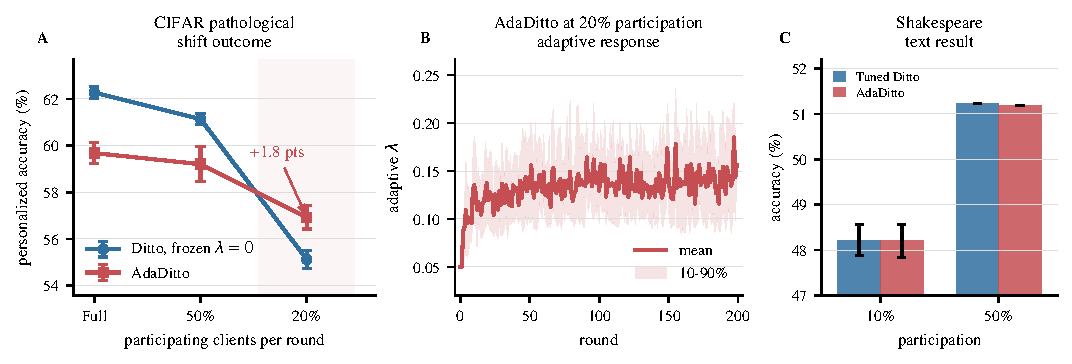
\includegraphics[width=0.95\textwidth]{Figures/current/shift_response.pdf}
  \caption{AdaDitto reduces coefficient staleness under participation shift. On CIFAR-100 pathological, the full-participation sweep selects $\lambda=0$; after shifting to 20\% participation, this frozen coefficient becomes stale, while AdaDitto increases coupling online and improves over the tune-once baseline by 1.8 points. The adaptive trajectory shows the learned coefficient rising during training. Shakespeare is a boundary case: AdaDitto matches tuned Ditto because the optimal nonzero coefficient is stable rather than shifted.}
  \label{fig:shift_outcome}
\end{figure*}

Relative to the target condition's best fixed coefficient, the stale
$\lambda=0$ choice incurs 4.7 points of regret, whereas AdaDitto
incurs 2.3 points. The full regret matrix, including cross-regime
stress cases, is reported in the supplementary material.

Table~\ref{tab:client-tail} shows that the gain extends to the client
tail. At 20\% participation,
AdaDitto improves client-unweighted 10th-percentile accuracy by
7.0 points and worst-client accuracy by 5.3 points over frozen
$\lambda=0$ Ditto.

\begin{table}[t]
\centering
\scriptsize
\setlength{\tabcolsep}{4pt}
\renewcommand{\arraystretch}{1.08}
\begin{tabularx}{\columnwidth}{@{}>{\raggedright\arraybackslash}Xcccc@{}}
\toprule
Method & Seeds & Mean & p10 & Worst \\
\midrule
Tune-once Ditto, $\lambda=0$ & 3 & 52.6 & 42.1 & 39.9 \\
AdaDitto & 3 & 55.8 & 49.2 & 45.3 \\
Ditto oracle, $\lambda=1$ & 3 & 58.7 & 53.6 & 50.0 \\
\bottomrule
\end{tabularx}
\caption{Client-tail personalized accuracy (\%) on CIFAR-pathological at 20\% participation, averaged on the common seed set \texttt{0,1,2}. Rows are client-unweighted final accuracies, unlike the headline Figure~\ref{fig:shift_outcome} aggregation.}
\label{tab:client-tail}
\end{table}

This tail table is intentionally stricter than the headline aggregate:
each client contributes equally within a run, so the statistic asks
whether the shift response helps difficult clients rather than only
raising the average sampled-client score. The common seed set removes
the seed-count mismatch between the tune-once, AdaDitto, and oracle
rows, while the oracle row shows that room remains between AdaDitto
and a freshly tuned fixed coefficient.

AdaDitto does not improve over the frozen baseline on CIFAR-100
practical, where participation shift does not create the same
coupling-regime failure. On Shakespeare, AdaDitto matches tuned
Ditto, but the optimal nonzero coefficient is stable, so the result
is parity rather than a shift win.

\subsection{The Loss-Gap Signal Tracks Increased Anchoring Need}

The adaptive trajectory in Figure~\ref{fig:shift_outcome} is
consistent with the fixed-coefficient sweep. On CIFAR-100
pathological under full participation, where the best fixed
coefficient is $\lambda=0$, the post-warmup mean loss gap is
0.013 and the learned coefficient is 0.090. Under 20\%
participation, where the sweep independently selects stronger
coupling, the mean loss gap rises to 0.074 and the learned
coefficient rises to 0.135.

Table~\ref{tab:mechanism-audit} connects the fixed-coefficient
optimum, controller signal, and learned coefficient.

\begin{table}[t]
\centering
\scriptsize
\setlength{\tabcolsep}{3pt}
\renewcommand{\arraystretch}{1.08}
\begin{tabularx}{\columnwidth}{@{}>{\raggedright\arraybackslash}Xccc@{}}
\toprule
Condition & Best fixed $\lambda$ & Mean gap & Mean learned $\lambda$ \\
\midrule
CIFAR-path full & 0.0 & 0.013 & 0.090 \\
CIFAR-path 20\% & 1.0 & 0.074 & 0.135 \\
Shakespeare 10\% & $>0$ & 0.003 & 0.069 \\
\bottomrule
\end{tabularx}
\caption{Mechanism audit connecting the fixed-coefficient sweep, controller signal, and learned coefficient.}
\label{tab:mechanism-audit}
\end{table}

The CIFAR-pathological shift raises both the gap and the learned
coefficient; Shakespeare instead shows floor-driven stable coupling.

\subsection{Controller Tuning Is Not the New Sweep}

A possible failure mode is that AdaDitto simply replaces a
$\lambda$ sweep with a brittle controller sweep. Figure~\ref{fig:controller_sensitivity}
tests this at the headline conditions. On CIFAR-100 pathological
with 20\% participation, all 11 tested controller configurations
beat the stale tune-once baseline, and the default configuration is
median-ranked rather than cherry-picked. On Shakespeare, all
11 configurations lie in a 0.03-point band and remain within
0.13 points of tuned Ditto.

\begin{figure*}[t]
  \centering
  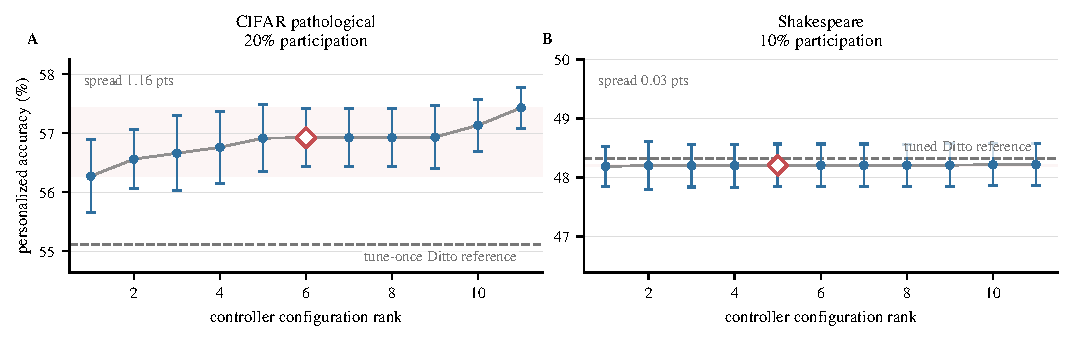
\includegraphics[width=0.95\textwidth]{Figures/current/controller_sensitivity.pdf}
  \caption{Controller sensitivity at the headline conditions. The white diamond marks the default controller, and the dashed line marks the fixed-Ditto reference for each panel. On CIFAR-100 pathological at 20\% participation, all 11 controller configurations beat the stale tune-once baseline, so the shift result does not depend on a cherry-picked default. On Shakespeare, all configurations lie in a 0.03-point band and remain within 0.13 points of tuned Ditto. Both panels average three seeds; error bars show standard deviation.}
  \label{fig:controller_sensitivity}
\end{figure*}

These scans do not show that controller parameters are irrelevant.
They show that the main conclusion does not depend on a lucky
default: the CIFAR-pathological shift result survives controller
variation, and the Shakespeare parity result remains insensitive.

We also ran controller ablations as a negative control. On
CIFAR-pathological, principled variants clustered near 0.597
personalized accuracy, while random adaptive coefficients fell to
0.5863. This separates useful loss-gap adaptation from arbitrary
adaptivity under high heterogeneity.

\subsection{Oracle Retuning, FedProx Nulls, and Shakespeare Parity}

The tune-once comparison is deployment-relevant, but it is weaker
than a per-condition oracle. When fixed Ditto is re-tuned separately
for each participation level, AdaDitto trails the tuned oracle by
roughly 1.4--2.6 points on CIFAR-100. AdaDitto should therefore
be read as a retuning-reduction mechanism, not as a replacement
for exhaustive per-condition tuning when such tuning is available.
This calibration matters because the oracle answers a different
question from the deployment experiment. The oracle assumes that the
target participation regime is already known and that enough
distributed runs are available to search it directly. The tune-once
setting instead asks what happens when a coefficient chosen before
deployment is reused after the operating point changes. AdaDitto's
value is in reducing the penalty caused by coefficient staleness, not
in beating a hindsight sweep that is allowed to spend a full run on
every candidate coefficient.

Per-condition oracle comparisons are reported in
Table~\ref{tab:oracle-comparison}.

\begin{table}[t]
\centering
\scriptsize
\setlength{\tabcolsep}{4pt}
\renewcommand{\arraystretch}{1.08}
\begin{tabular}{@{}lccc@{}}
\toprule
Split & Part. & Ditto & AdaDitto \\
\midrule
practical & 50\% & 48.2 & 46.1 \\
practical & 20\% & 47.0 & 44.4 \\
pathological & 50\% & 61.0 & 59.2 \\
pathological & 20\% & 58.7 & 57.2 \\
\bottomrule
\end{tabular}
\caption{CIFAR-100 personalized accuracy (\%) against per-condition tuned Ditto, averaged over five seeds. The oracle re-tunes the coefficient for each condition; this is the upper bound AdaDitto is not claiming to replace.}
\label{tab:oracle-comparison}
\end{table}

FedProx is a negative probe: across tested CIFAR-100 settings,
$\mu=0$ or near-zero remains best. In additional FedProx probes
outside the final Ditto protocol, this remains true even with five
local epochs and 20\% participation, so AdaFedProx has no useful
proximal signal to recover. Shakespeare is a boundary case:
$\lambda=0$ is poor, nonzero coupling is stable across 10\% and
50\% participation, and AdaDitto matches tuned Ditto rather than
producing a shift win.

The FedProx null results and the Shakespeare boundary case are
summarized in Table~\ref{tab:null-boundary}.

\begin{table}[tbp]
\centering
\scriptsize
\setlength{\tabcolsep}{3pt}
\renewcommand{\arraystretch}{1.08}
\begin{tabularx}{\columnwidth}{@{}>{\raggedright\arraybackslash}p{0.19\columnwidth}>{\raggedright\arraybackslash}p{0.15\columnwidth}>{\raggedright\arraybackslash}p{0.29\columnwidth}>{\raggedright\arraybackslash}X@{}}
\toprule
Dataset & Method & Setting & Outcome \\
\midrule
CIFAR-100 & FedProx & $E=1$, full participation & small or zero $\mu$ best \\
CIFAR-100 & FedProx & $E=5$, full participation & $\mu=0$: 63.5; $\mu=1$: 57.1 \\
CIFAR-100 & FedProx & $E=5$, 20\% participation & $\mu=0$: 23.0; $\mu>0$: 19.6 \\
CIFAR-100 & FedProx & $E=5$, 20\% + systems heterogeneity & $\mu=0$: 25.9; $\mu=1$: 22.2 \\
Shakespeare & Ditto & 10\% / 50\%, $\lambda=0$ & 34.4 / 44.5 \\
Shakespeare & Ditto & 10\% / 50\%, $\lambda=0.1$ & 48.3 / 51.2 \\
\bottomrule
\end{tabularx}
\caption{Null and boundary probes. CIFAR-100 FedProx results show no useful positive-$\mu$ regime, while Shakespeare Ditto results show that nonzero coupling is beneficial but stable across 10\% and 50\% participation. Values are personalized accuracy (\%).}
\label{tab:null-boundary}
\end{table}

\subsection{Runtime and Communication Overhead}

AdaDitto preserves Ditto's model-update communication pattern. Each
participating client sends one scalar probe loss, and the server
broadcasts one scalar reference loss in the next round; no extra model,
gradient, optimizer state, or client-to-client message is introduced.
Computation adds only a no-gradient forward pass on a probe minibatch
containing 10\% of local training examples, capped at 256. Thus the
per-round overhead is scalar bookkeeping plus a small local probe,
while static retuning requires full distributed runs for each candidate
$\lambda$.

\subsection{Reproducibility and Reporting}

All reported experiments are implemented as modifications to
PFLlib~\cite{zhang2025pfllib}. CIFAR-100 is obtained from the public
CIFAR distribution; Shakespeare is obtained through the public LEAF
preprocessing pipeline~\cite{caldas2018leaf}. Raw datasets are not
redistributed. The anonymized code archive is linked in the main paper,
and the experiment scripts and run artifacts record the command lines,
configuration files, environment snapshots, and per-run metrics used
to generate the figures.

The final model and optimization settings are summarized in
Table~\ref{tab:training-protocol}.

\begin{table}[t]
\centering
\scriptsize
\setlength{\tabcolsep}{3pt}
\renewcommand{\arraystretch}{1.08}
\begin{tabularx}{\columnwidth}{@{}>{\raggedright\arraybackslash}p{0.23\columnwidth}cc>{\raggedright\arraybackslash}X@{}}
\toprule
Dataset & Model & Rounds & Clients / optimizer \\
\midrule
CIFAR practical & CNN & 200 & 20 clients, full/50\%/20\%, SGD lr 0.01 \\
CIFAR pathological & CNN & 200 & 20 clients, full/50\%/20\%, SGD lr 0.01 \\
Shakespeare & char-LSTM & 40 & 118 clients, 10\%/50\%, SGD lr 0.5 \\
\bottomrule
\end{tabularx}
\caption{Final training protocol. All rows use one local epoch, batch size 64, and no weight decay. Ditto and AdaDitto train global and personalized models with the same local learning rate.}
\label{tab:training-protocol}
\end{table}

For multi-seed comparisons, CIFAR core runs use seeds
\texttt{0,1,2,3,4}. Tune-once shift tests, Shakespeare core
comparisons, and controller stress scans use seeds \texttt{0,1,2}.
Single-seed sweeps are used only to identify coefficient regimes, not
as significance claims. Each run applies the seed before data
partitioning, model initialization, client sampling, and minibatch
shuffling; paired comparisons reuse the same seed set when methods are
compared directly.

We do not use null-hypothesis significance tests for the main claims.
Instead, we separate roles: single-seed sweeps expose coefficient
regimes; multi-seed core comparisons estimate robustness; controller
stress scans test whether the default is lucky; and the random-adaptive
ablation serves as a negative control. This reporting structure is meant to make the
limits of the claim visible: AdaDitto reduces coefficient staleness
under deployment shift, but it is not presented as a universal
replacement for oracle retuning.

\subsection{Limitations}

The controller's lower bound is load-bearing. When the best fixed
coefficient is truly near zero, as in CIFAR-pathological full
participation, AdaDitto cannot reduce $\lambda$ below
$\lambda_{\min}=0.05$ and therefore slightly over-anchors relative to
the pure-local optimum. This is a deliberate safety choice, but it
means the method should not be read as an exact online optimizer for
$\lambda$. It is a bounded controller that limits losses caused by
coefficient staleness, not a mechanism that recovers every per-condition
optimum.

The loss-gap signal is most informative under the CIFAR participation
shift, where larger gaps coincide with the fixed-coefficient sweep
moving toward stronger anchoring. Shakespeare exposes a different
boundary case: the gap is nearly zero, while nonzero coupling remains
important. AdaDitto matches tuned Ditto there largely because the
lower-bound floor supplies stable coupling, not because the gap detects
a shift. This distinction scopes the mechanism: active gap-driven
adaptation helps when deployment increases anchoring need, while the
floor mainly protects regimes with consistently nonzero coupling.

Finally, the present study uses controlled CIFAR splits and a LEAF
Shakespeare check rather than a broad production deployment. We vary
participation and heterogeneity, but do not yet study device churn,
asynchronous updates, privacy accounting for probe losses, larger
language models, or multimodal clients. Those settings may require
additional safeguards around probe sampling, coefficient sharing, or
privacy-preserving loss reporting.

The main conclusion would weaken under two concrete outcomes. First,
if a broader benchmark suite showed that participation shifts rarely
change the preferred coupling regime, then coefficient staleness would
be less practically important. Second, if privacy or systems
constraints made even scalar probe-loss reporting unavailable, then
AdaDitto would need a different stress signal. These are deployment
questions rather than formatting details: the present evidence supports
bounded online proximal control for the tested shifts, not a universal
claim about all personalization regimes.

\section{Conclusion}

We studied proximal coefficient selection as a deployment-stability
problem rather than a one-time tuning problem. Fixed Ditto
coefficients can encode the wrong coupling regime after
participation shift: on CIFAR-100 pathological, the
full-participation choice $\lambda=0$ becomes stale under 20\%
participation. AdaDitto uses a bounded loss-gap controller to
increase coupling online, reducing the resulting coefficient staleness
while preserving the underlying Ditto objective form and model-update
communication pattern.

Proximal sweeps diagnose coupling regimes; they do not certify
deployment safety.

\bibliography{references}
% \input{ReproducibilityChecklist.tex}

\end{document}
